\section{Questions sur le chapitre ``Transferts et échangeurs de chaleur''}
\subsection{Expliquez de façon concise les 3 modes de transfert de chaleur.}
\begin{description}
	\item[La conduction] est un mode de transfert thermique provoqué par un gradient de température entre deux régions d'un même milieu ou entre deux milieux en contact. Elle résulte des interactions entre particules voisines, collisions pour les fluides et vibration pour les solides. 
	\item[La convection] est un transfert thermique qui s'accompagne du mouvement de molécules dans un fluide.
	\item[Le rayonnement] est un transfert thermique qui s'effectue par le rayonnement électromagnétique. Le transfert peut se réaliser sans présence de matière.
\end{description}

\subsection{Dérivez l'équation de la diffusion thermique d'un corps non-déformable et au repos.}
Selon la \textbf{loi de Fourier}, le flux de chaleur $\vec{q}$ en un point est une fonction linéaire du gradient de température en ce point :
\begin{equation} \vec{q} = -k\grad T \label{eq:fourier}\end{equation}
où $k$ est la conductibilité du milieu.
Considérons un corps non-déformable et au repos. Appelons $V$ et $A$ respectivement le volume et la frontière du corps. Évidemment $V=C^\text{te}$ et $A=C^\text{te}$. De plus, appelons $e$ l'énergie interne spécifique du corps. On suppose que $e$ ne dépend que de la température :
\begin{equation} de = cdT \label{eq:efonctiondeT}\end{equation}
avec $c$ la chaleur massique du corps. Étant donné que le coprs est non-déformable et au repos, la vitesse de chaque point matériel du corps est nulle :
\begin{equation} \vec{u} = 0 \label{eq:vitesse_nulle}\end{equation}
Ceci implique que l'énergie cinétique du corps est nulle. Par conséquent, le corps ne peut échanger que de la chaleur avec son environnement. Le bilan d'énergie prend donc la forme suivante :
\begin{equation} \frac{\partial}{\partial t}\int_V\rho edV = - \int_A\vec{q}\cdot\vec{n}dA + \int_Vq_rdV \end{equation}
avec dans cette équation $\rho$ la masse volumique, $\vec{n}$ le vecteur unitaire et perpendiculaire à la frontière $A$ et $q_r$ la chaleur ajoutée au corps par des sources ou des fuites d'énergie (\si{\watt\per\metre\cubed}). Étant donné que le volume $V$ du corps est constant, nous constatons que la dérivée temporelle peut être mise à l'intérieur de l'intégrale. De plus, on peut appliquer le théorème de la divergence à l'intégrale du flux de chaleur :
\begin{equation} \int_V\frac{\partial}{\partial t}(\rho e)dV = -\int_V\grad\cdot\vec{q}dV + \int_Vq_rdV \end{equation}
Cette équation doit être valable pour un volume arbitraire, ce qui implique
\begin{equation} \frac{\partial}{\partial t}(\rho e) = -\grad\cdot\vec{q} + q_r \end{equation}
En appliquant \ref{eq:fourier}, la loi de Fourier :
\begin{equation} \frac{\partial}{\partial t}(\rho e) = \grad\cdot(k\grad T) + q_r \label{eq:appfourier}\end{equation}
De plus, si nous tenons compte de l'équation de la conservation de la masse et de l'équation \ref{eq:vitesse_nulle} :
\begin{equation} \frac{\partial\rho}{\partial t} + \grad\cdot(\rho\vec{u}) = 0 \qquad \Rightarrow \qquad \frac{\partial\rho}{\partial t} = 0 \label{eq:conservationmasse}\end{equation}
La combinaison des équations \ref{eq:efonctiondeT} et \ref{eq:vitesse_nulle} nous donne :
\begin{equation} de = cdT \Rightarrow \frac{de}{dt} = c\frac{dT}{dt} \Rightarrow \frac{\partial e}{\partial t} = c\frac{\partial T}{\partial t} \label{eq:decdT}\end{equation}
Finalement, la combinaison des équations \ref{eq:appfourier}, \ref{eq:conservationmasse} et \ref{eq:decdT} nous donne l'équation de diffusion thermique
\begin{equation} \rho c\frac{\partial T}{\partial t} = k\grad^2T + q_r \label{eq:chaleur}\end{equation}
dans le cas spécial où $k = C^\text{te}$.

\subsection{Dérivez la distribution de température dans une paroi plane. La longueur de la paroi est infinie, son épaisseur est constante, ses surfaces extérieures sont maintenues à des températures constantes et les propriétés de la paroi sont homogènes.}
En régime stationnaire et en l'absence de source volumique de chaleur, l'équation de chaleur \ref{eq:chaleur} se réduit à :
\begin{equation} \grad^2T = 0 \end{equation}
dont l'intégration nous donne dans le cas d'un problème unidimensionnel (figure \ref{fig:q3_3}) :
\begin{equation} T = Ax+B \end{equation}
Si nous prenons comme conditions limites :
\begin{equation} \begin{cases} T(x=0) &= T_1 \\ T(x=e) &= T_2 \end{cases} \qquad \Rightarrow \qquad \begin{cases} A &= \frac{T_2-T_1}{e} \\ B &= T_1 \end{cases} \end{equation}
L'équation du champ thermique devient donc :
\begin{equation} T = \frac{T_2-T_1}{e}x+T_1 \end{equation}
Par la loi de Fourier :
\begin{align} \dot{q} &= -k\grad T \\ &= \frac{k}{e}(T_1-T_2) \end{align}
Si la paroi sépare deux milieux continus à des températures $T_{f1}$ et $T_{f2}$, alors la continuité du flux de chaleur impose :
\begin{equation} \dot{q} = h_1(T_{f1}-T_1) = \frac{k}{e}(T_1-T_2) = h_2(T_2-T_{f2}) \end{equation}
où $h_1$ et $h_2$ désignent les coefficients de convection relatifs au contact des deux fluides avec la paroi $[\si{\watt\per\meter\squared\per\kelvin}]$.
\begin{figure}[p]\centering
	\tikzsetnextfilename{q3_3}
    \begin{tikzpicture}
        \draw (0,0) -- (0,5);
    	\fill[pattern=north west lines] (0,0) rectangle ++(0.2,5); 
	    \draw (2,0) -- (2,5);
	    \fill[pattern=north west lines] (2,0) rectangle ++(-0.2,5); 
	    
	    \draw[->] (-3,-1) -- (-3,6) node[above]{$T$};
	    \draw[->] (-3,-1) -- (4,-1) node[right]{$x$};
		\draw[red,thick] (-2.8,4) -- (-2.5,4) -- (0,3) -- (2,2) -- (3,1) -- (3.5,1);
		\draw[red,dashed] (-2.5,4) to[out=0,in=110] (0,3);
		\draw[red,dashed] (2,2) to[out=-90,in=180] (3,1);
		\draw (0,3) node{$\circ$};
		\draw (0,3) node[below left]{$T_1$};
		\draw (2,2) node{$\circ$};
		\draw (2,2) node[above right]{$T_2$};
		\draw (-2.5,4) node{$\circ$};
		\draw (-2.5,4) node[above]{$T_{f1}$};
		\draw (3,1) node{$\circ$};
		\draw (3,1) node[above right]{$T_{f2}$};
		
		\draw[<->] (0,-0.5) -- (2,-0.5) node[midway,above]{$e$};
		\draw[<->] (-2.5,-0.5) -- (0,-0.5) node[midway,above]{$\frac{k}{h_1}$};
		\draw[<->] (2,-0.5) -- (3,-0.5) node[midway,above]{$\frac{k}{h_2}$};
		\draw (-1.5,5) node{$h_1$};
		\draw (1,5) node{$\frac{k}{e}$};
		\draw (3,5) node{$h_2$};
		

    \end{tikzpicture}
    \caption{Distribution de température dans une paroi plane}
    \label{fig:q3_3}
\end{figure}

\subsection{Dérivez l'expression du coefficient de transmission globale $U$ pour une paroi plane composée qui comprend $n$ plaques en contact.}
En pratique on exprime le flux de chaleur $\vec{q}$ en fonction d'un coefficient de transmission $U$ global et des température $T_{f1}$ et $T_{f2}$ :
\begin{equation} \dot{q} = U(T_{f1} - T_{f2}) \end{equation}
Le coefficient $U$ a les mêmes dimensions que $h$. Il s'exprime donc en \si{\watt\per\meter\squared\per\kelvin}. Par la continuité du flux de chaleur on a :
\begin{align} \dot{q} &= h_1(T_{f1}-T_1) = \frac{k_n}{e_n}(T_n-T_{n+1}) = h_2(T_{n+1} - T_{f2}) \\ &= \frac{T_{f1}-T_1}{\frac{1}{h_1}} = \frac{T_1-T_2}{\frac{e_1}{k_1}} = \ldots = \frac{T_n-T_{n+1}}{\frac{e_n}{k_n}} = \frac{T_{n+1}-T_{f2}}{\frac{1}{h_2}} \\ &= \frac{T_{f1}-T_{f2}}{\frac{1}{h_1} + \sum_i^n\frac{e_i}{k_i} + \frac{1}{h_2}} = \frac{T_{f1} - T_{f2}}{\frac{1}{U}}\end{align}
Ceci définit le coefficient de transmission global $U$ :
\begin{equation} \frac{1}{U} = \frac{1}{h_1} + \sum_i^n\frac{e_i}{k_i} + \frac{1}{h_2} \end{equation}

\subsection{Dérivez la distribution de température dans une paroi cylindrique simple. l'étendue de la paroi est infinie, ses surfaces extérieures sont maintenues à des températures constantes et les propriétés de la paroi sont homogènes.}
En régime stationnaire et en l'absence de source volumique de chaleur, l'équation de chaleur \ref{eq:chaleur} se réduit à :
\begin{equation} \grad^2T = 0 \end{equation}
En coordonnées cylindriques cela donne :
\begin{align} \frac{d^2T}{dr^2} + \frac{1}{r}\frac{dT}{dr} = 0 \qquad&\Leftrightarrow\qquad rdT' + T'dr = 0 \\ &\Leftrightarrow\qquad rT' = A \\ &\Leftrightarrow\qquad \frac{dT}{dr} = \frac{A}{r} \end{align}
Par une seconde intégration, on trouve :
\begin{equation} T = A\ln{r} + B \end{equation}
Si nous prenons comme conditions limites
\begin{equation} \begin{cases} T(r=r_i) &= T_i \\ T(r=r_e) &= T_e \end{cases} \qquad \Rightarrow \qquad \begin{cases} T_i &= A\ln{r_i} + B \\ T_e &= A\ln{r_e} + B \end{cases} \end{equation}
on obtient 
\begin{equation} T = \frac{T_i - T_e}{\ln\frac{r_i}{r_e}}\ln{r} + \frac{T_e\ln{r_i} - T_i\ln{r_e}}{\ln\frac{r_i}{r_e}} \label{eq:paroi_cylindrique}\end{equation}
Le profil de température à travers la paroi cylindrique est disponible à la figure \ref{fig:q3_5}
\begin{figure}[p]\centering
	\tikzsetnextfilename{q3_5}
    \begin{tikzpicture}
        \draw (1,0) node[below]{$r_i$} -- (1,5);
    	\fill[pattern=north west lines] (1,0) rectangle ++(0.2,5); 
	    \draw (4,0) node[below]{$r_e$} -- (4,5);
	    \fill[pattern=north west lines] (4,0) rectangle ++(-0.2,5); 
	    
	    \draw[->] (0,0) -- (0,6) node[above]{$T$};
	    \draw[->] (0,0) -- (5,0) node[right]{$r$};
		\draw (1,4) node{$\circ$};
		\draw (1,4) node[below left]{$T_i$};
		\draw (4,1) node{$\circ$};
		\draw (4,1) node[above right]{$T_e$};
		
		\draw[domain=1:4,smooth,variable=\x,red,thick] plot ({\x},{-2.164*ln(\x) + 4});
    \end{tikzpicture}
    \caption{Distribution de température dans une paroi cylindrique}
    \label{fig:q3_5}
\end{figure}

\subsection{Dérivez l'expression du rayon critique d'une paroi cylindrique simple}
L'équation explicite du champ thermique à travers une paroi cylindrique \ref{eq:paroi_cylindrique} nous montre que le gradient de température est :
\begin{equation} \grad T = \frac{dT}{dr} = \frac{T_i-T_e}{\ln\frac{r_i}{r_e}}\frac{1}{r} \end{equation}
Le flux, calculé pour une longueur $l$ de la paroi vaut :
\begin{equation} \dot{Q} = S\dot{q} = 2\pi rlk\frac{T_i-T_e}{\ln\frac{r_i}{r_e}}\frac{1}{r} \end{equation}
fa continuité du flux nous indique que celui-ci est indépendant du rayon $r$. En faisant usage des conditions aux frontières :
\begin{equation} \begin{cases} \dot{Q}(r=r_i) &= 2\pi r_ilh_i(T_{fi}-T_i) \\ \dot{Q}(r=r_e) &= 2\pi r_elh_e(T_e-T_{fe}) \end{cases} \end{equation}
où $T_{fi}$ et $T_{fe}$ représente respectivement les températures loin de paroi intérieure et de la paroi extérieure.
On peut exprimer le flux en fonction d'un coefficient de transmission global $U_i$ ou $U_e$ défini par les relations :
\begin{equation} \dot{Q} = U_iS_i(T_{fi}-T_{fe}) = U_eS_e(T_{fi}-T_{fe}) \end{equation}
En effet, on peut écrire :
\begin{equation} \dot{Q} = \frac{T_{fi}-T_i}{\frac{1}{h_iS_i}} = \frac{T_i-T_e}{\frac{1}{2\pi lk}\ln\frac{r_e}{r_i}} = \frac{T_e - T_{fe}}{\frac{1}{h_eS_e}} = \frac{T_{fi}-T_{fe}}{\frac{1}{h_iS_i} + \frac{1}{2\pi lk}\ln\frac{r_e}{r_i} + \frac{1}{h_eS_e}} \end{equation}
Il en résulte donc :
\begin{equation} \frac{1}{U_iS_i} = \frac{1}{U_eS_e} = \frac{1}{h_iS_i} + \frac{1}{2\pi lk}\ln\frac{r_e}{r_i} + \frac{1}{h_eS_e} \end{equation}
On va se concentrer sur $U_i$ mais on peut très bien effectuer un raisonnement similaire sur $U_e$. Si $r_i$, $h_i$ et $h_e$ sont fixés, $1/U_i$ est fonction du rayon extérieur $r_e$ :
\begin{equation} \frac{1}{U_i} = \frac{1}{h_i} + \frac{r_i}{k}\ln\frac{r_e}{r_i} + \frac{1}{h_e}\frac{r_i}{r_e} \end{equation}
Cette fonction se compose de la somme d'un terme constant ($\frac{1}{h_i}$), d'une fonction croissante ($\frac{r_i}{k}\ln\frac{r_e}{r_i}$) et d'une fonction décroissante ($\frac{r_i}{h_er_e}$). Elle présente un minimum pour une valeur de $r_e$ que l'on appelle le rayon critique $r_c$ :
\begin{equation} \frac{d}{dr_e}\left(\frac{1}{U_i}\right) = \frac{r_i}{kr_e} - \frac{r_i}{h_er_e^2} = 0 \qquad \Rightarrow \qquad r_c = \frac{k}{h_e} \end{equation}
Le rayon critique est donc le rayon extérieur pour lequel le flux de chaleur est maximal. 

Envisageons le cas particulier d'un tube isolant placé dans l'air, condition dans laquelle on a normalement $h_e \simeq \SI{10}{\watt\per\meter\squared\per\kelvin}$ et $k \simeq \SI{0.05}{\watt\per\meter\per\kelvin}$. Si on trace la fonction de ($\frac{1}{U_i}$) en fonction de $r_e$ on obtient la figure \ref{fig:q3_6}. Dans le cas d'un tube isolant, on cherche à minimiser la déperdition calorifique. Pour cela on va essayer de rester en deçà du rayon critique en rendant le tube aussi mince que possible. Ce paradoxe provient du fait qu'en diminuant le rayon extérieur, on diminue la résistance liée à la conduction mais on augment aussi celle liée à la convection externe.
\begin{figure}[p]\centering
	\tikzsetnextfilename{rayon_critique_isolant}
    \begin{tikzpicture}
        \begin{axis}[
        	enlargelimits=true,
        	axis lines=left, xtick=\empty, ytick=\empty,
        	grid=major,
        	xmax = 0.025,
        	ymin = -0.02,
        	ylabel=$\frac{1}{U_i}\;(\si{\meter\squared\kelvin\per\watt})$,
        	xlabel=$r_e\;(\si{\meter})$,
        	legend style={font=\footnotesize},
        	xtick={0,0.01,0.015,0.02,0.025},
		    xticklabels={$0$,$1$,$1.5$,$2$,$2.5$},
		    ytick={0,0.05,0.1,0.2},
		    yticklabels={$0$,$0.05$,$0.1$,$0.2$},
    		extra x ticks=0.005,
		    extra x tick style={grid=major, grid style={dashed,black}},
		    extra x tick labels={$r_c$},
    		extra y ticks=0.1522,
		    extra y tick style={grid=major, grid style={dashed,black}},
		    extra y tick labels={$(1/U_1)_\text{min}$}
		]
            \addplot [thick,domain=0.001:0.02,samples=200] {0.1 + 0.02*ln(x/0.001) + 0.0001/x} node[right,pos=1] {$\frac{1}{U_i}$};;
            \addplot [domain=0.001:0.02,samples=200] {0.02*ln(x/0.001)} node[right,pos=1] {$\frac{r_i}{k}\ln\frac{r_e}{r_i}$};
            \addplot [domain=0.001:0.02,samples=200] {0.0001/x} node[right,pos=1] {$\frac{1}{h_e}\frac{r_i}{r_e}$};
        \end{axis}
    \end{tikzpicture}
    \caption{Rayon critique dans le cas d'un tube isolant}
    \label{fig:q3_6}
\end{figure}

\subsection{Dérivez les expressions de deux coefficients de transmission globaux $U_i$ et $U_e$ pour une paroi cylindrique qui se compose de $n$ couches concentriques en contact.}
Si la paroi cylindrique se compose de $n$ couches concentriques en contact, de conductibilités respectives $k_1$, $k_2$, $\ldots$, $k_n$, limitées par les rayons $r_i = r_1$, $r_2$, $\ldots$, $r_n$, $r_{n+1} = r_e$ où $r_i$ désigne le rayon intérieur et $r_e$ le rayon extérieur, on peut écrire pour chaque couche l'expression :
\begin{equation} \dot{Q} = 2\pi lk_j\frac{T_j-T_{j+1}}{\ln\frac{r_{j+1}}{r_j}} \qquad \text{pour } 1\leq j\leq n \end{equation}
De plus, on a :
\begin{equation} \dot{Q} = h_iS_i(T_{fi}-T_1) = h_eS_e(T_{n+1} - T_{fe}) \end{equation}
Dès lors,
\begin{equation} \dot{Q} = \frac{T_{fi}-T_1}{\frac{1}{h_iS_i}} = \ldots = \frac{T_j-T_{j+1}}{\frac{1}{2\pi lk_j}\ln\frac{r_{j+1}}{r_j}} = \ldots = \frac{T_{n+1}-T_{fe}}{\frac{1}{h_eS_e}} = \frac{T_{fi}-T_{fe}}{\frac{1}{U_iS_i}} \end{equation}
On trouve ainsi :
\begin{align} \frac{1}{U_i} &= \frac{1}{h_i} + r_i\sum_j\frac{1}{k_j}\ln\frac{r_{j+1}}{r_j} + \frac{1}{h_e}\frac{r_i}{r_e} \\ \frac{1}{U_e} &= \frac{1}{h_i}\frac{r_e}{r_i} + r_e\sum_j\frac{1}{k_j}\ln\frac{r_{j+1}}{r_j} + \frac{1}{h_e} \end{align}

\subsection{Donnez la définition de débit de capacité calorifique d'un fluide dans un échangeur de chaleur.}
Désignons respectivement par $\dot{M}^x$ et $\dot{M}^0$ les débits massiques des fluides chauffant et chauffé le long de la surface de chauffe, par $T^x$ la température du fluide chauffant et par $T^0$ la température du fluide chauffé. Les indices $1$ et $2$ se rapportent respectivement à l'entrée et à la sortie des fluides dans l'échangeur.

Nous appellerons débit de capacité calorifique d'un fluide le produit $\dot{M}c$ de ce fluide, soit le produit du débit massique et de la capacité calorifique. Les écarts entre $T_1^x$ et $T_2^x$ d'une part, et entre $T_1^0$ et $T_2^0$ d'autre part, sont en pratique suffisamment faibles pour que les chaleurs massiques $c^x$ et $c^0$ puissent être considérées comme constantes.

On considérera également comme constant le coefficient de transmission total à travers la paroi et l'on supposera nulle toute perte calorifique extérieure.

\subsection{Dérivez l'expression pour la distribution de température du fluide chauffant d'un évaporateur co-courant.}
La puissance calorifique $d\dot{Q}$ échangée à travers un élément de surface $dS$ est :
\begin{equation} d\dot{Q} = -\dot{M}^xc^xdT^x = \dot{M}^0c^0dT^0 = U(T^x-T^0)dS \end{equation}
Les signes se justifient par le fait que pour $dS > 0$, on aura $dT^x < 0$ et $dT^0 > 0$. L'évaporateur est un cas particulier d'échangeur de chaleur car la température du fluide chauffé reste constante : $dT^0 = 0$
Dans ce cas, on a :
\begin{equation} \dot{Q} = \dot{M}^xc^x(T_1^x - T_2^x) \end{equation}
et
\begin{equation} \frac{dT^x}{T^x-T^0} = \frac{d(T^x-T^0)}{T^x-T^0} = -\frac{U}{\dot{M}^xc^x}dS \end{equation}
ce qui nous donne :
\begin{align} \ln({T^x-T^0}) &= -\frac{U}{\dot{M}^xc^x}S + C\\
			\Leftrightarrow T^x-T^0 &= C\exp\left(-\frac{U}{\dot{M}^xc^x}S\right) \\
			& \qquad\text{en } S = 0 \text{ on a } T^x-T^0 = T_1^x-T_1^0 \\
			&\Rightarrow C = T_1^x-T^0 \\
			\Leftrightarrow\frac{T^x-T^0}{T_1^x-T^0} &= \exp\left(-\frac{U}{\dot{M}^xc^x}S\right)
\end{align}
Les distributions de température des fluides chauffant $T^x$ et chauffé $T^0$ sont représentées à la figure \ref{fig:q3_9}.
\begin{figure}[p]\centering
	\tikzsetnextfilename{evaporateur_co_courant}
    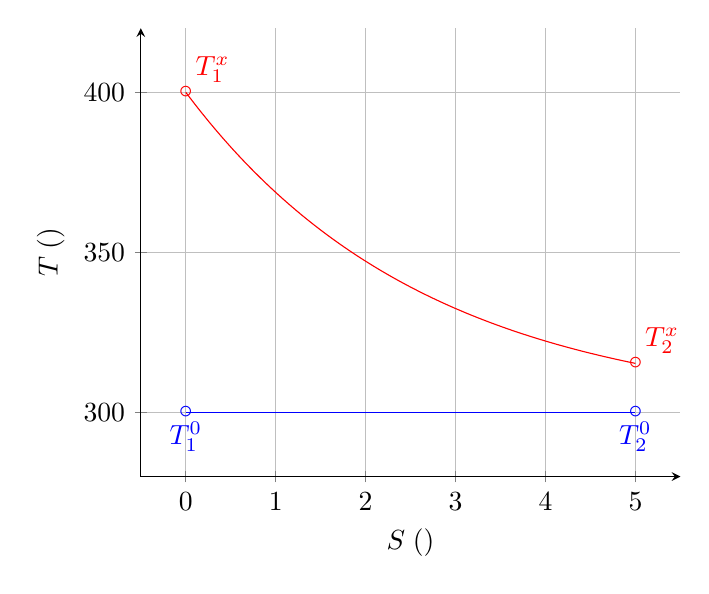
\begin{tikzpicture}
        \begin{axis}[
        	enlargelimits=true,
        	axis lines=left,
        	grid=major,
        	xmin = -0.5, xmax = 5.5,
        	ymin = 280, ymax = 420,
        	ylabel=$T\;(\si{\kelvin})$,
        	xlabel=$S\;(\si{\meter\squared})$,
		]
            \addplot [red,domain=0:5,samples=200] {(100*exp(-0.375*x)) + 300} node[pos=0] {$\circ$} node[above right,pos=0] {$T_1^x$} node[pos=1] {$\circ$} node[above right,pos=1]{$T_2^x$};
            \addplot [blue,domain=0:5,samples=200] {300} node[pos=0] {$\circ$} node[below,pos=0] {$T_1^0$} node[pos=1] {$\circ$} node[below,pos=1]{$T_2^0$};
        \end{axis}
    \end{tikzpicture}
    \caption{Distributions de température dans un évaporateur co-courant}
    \label{fig:q3_9}
\end{figure}

\subsection{Dérivez l'expression pour la distribution de température du fluide chauffé d'un condenseur co-courant.}
La puissance calorifique $d\dot{Q}$ échangée à travers un élément de surface $dS$ est :
\begin{equation} d\dot{Q} = -\dot{M}^xc^xdT^x = \dot{M}^0c^0dT^0 = U(T^x-T^0)dS \end{equation}
Les signes se justifient par le fait que pour $dS > 0$, on aura $dT^x < 0$ et $dT^0 > 0$. Le condenseur est un cas particulier d'échangeur de chaleur car la température du fluide chauffant reste constante : $dT^x = 0$
Dans ce cas, on a :
\begin{equation} \dot{Q} = \dot{M}^0c^0(T_2^0 - T_1^0) \end{equation}
et
\begin{equation} \frac{dT^0}{T^x-T^0} = -\frac{d(T^x-T^0)}{T^x-T^0} = \frac{U}{\dot{M}^0c^0}dS \end{equation}
ce qui nous donne :
\begin{align} \ln({T^x-T^0}) &= -\frac{U}{\dot{M}^0c^0}S + C\\
			\Leftrightarrow T^x-T^0 &= C\exp\left(-\frac{U}{\dot{M}^0c^0}S\right) \\
			& \qquad\text{en } S = 0 \text{ on a } T^x-T^0 = T_1^x-T_1^0 \\
			&\Rightarrow C = T^x-T_1^0 \\
			\Leftrightarrow\frac{T^x-T^0}{T^x-T_1^0} &= \exp\left(-\frac{U}{\dot{M}^0c^0}S\right)
\end{align}
Les distributions de température des fluides chauffant $T^x$ et chauffé $T^0$ sont représentées à la figure \ref{fig:q3_10}.
\begin{figure}[p]\centering
	\tikzsetnextfilename{condenseur_co_courant}
    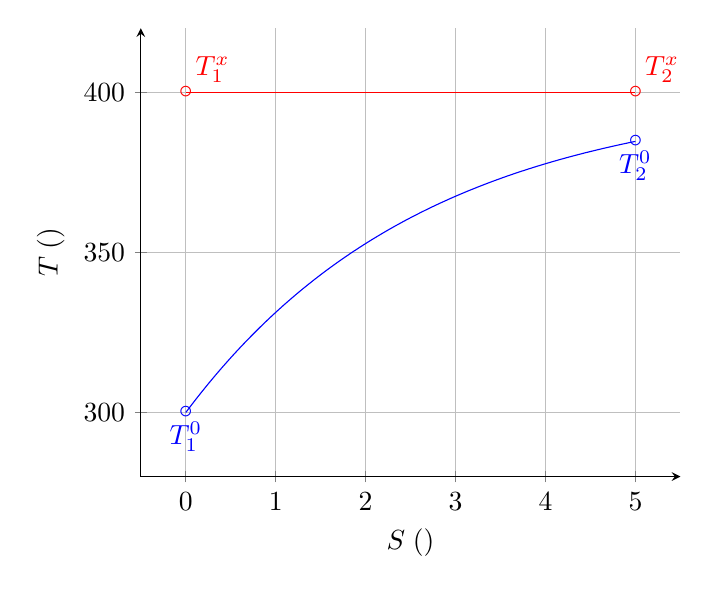
\begin{tikzpicture}
        \begin{axis}[
        	enlargelimits=true,
        	grid=major,
        	axis lines=left,
        	xmin = -0.5, xmax = 5.5,
        	ymin = 280, ymax = 420,
        	ylabel=$T\;(\si{\kelvin})$,
        	xlabel=$S\;(\si{\meter\squared})$,
		]
            \addplot [blue,domain=0:5,samples=200] {-(100*exp(-0.375*x)) + 400} node[pos=0] {$\circ$} node[below,pos=0] {$T_1^0$} node[pos=1] {$\circ$} node[below ,pos=1]{$T_2^0$};
            \addplot [red,domain=0:5,samples=200] {400} node[pos=0] {$\circ$} node[above right,pos=0] {$T_1^x$} node[pos=1] {$\circ$} node[above right,pos=1]{$T_2^x$};
        \end{axis}
    \end{tikzpicture}
    \caption{Distributions de température dans un condenseur co-courant}
    \label{fig:q3_10}
\end{figure}

\subsection{Expliquez le principe de fonctionnement d'un échangeur à fonctionnement non-continu à contact direct.}
\textbf{Un échangeur à fonctionnement non-continu à contact direct} est un échangeur où l'échange calorifique s'obtient par mélange de deux fluides. Le réchauffage d'un liquide peut être réalisé en y injectant de la vapeur, généralement de la vapeur d'eau. Cette méthode n'est applicable que si la condensation de la vapeur n'entraîne pas d'inconvénient pour le liquide. Ce procédé peut être utilisé, par exemple, pour la préparation d'eau chaude, ou pour permettre le déroulement d'une réaction chimique nécessitant une température élevée.

\subsection{Expliquez le principe de fonctionnement d'un échangeur à fonctionnement non-continu et à contact indirect.}
\textbf{Un échangeur à fonctionnement non-continu à contact indirect} est un échangeur dans lequel le liquide est progressivement réchauffé ou refroidi avant d'être évacué. Il existe différents procédés :
\begin{itemize}
\item chauffage électrique (boilers, ceux-ci peuvent aussi fonctionner en régime continu),
\item serpentin immergé dans la cuve dans lequel circule le fluide chauffant ou réfrigérant,
\item cuve à double fond.
\end{itemize}
Dans chacun de ces procédés, il convient d'agiter le fluide afin d'obtenir une répartition uniforme de la température.
